%%%
%%%  ŠABLONA PRO BAKALÁŘSKOU PRÁCI MFF UK - MATEMATIKA
%%%
%%%  * hlavní soubor (Masterfile)
%%%
%%%  Tato šablona předpokládá kompilaci souboru pomocí sekvence:
%%%    cslatex -> bibtex -> cslatex (2x) -> dvips -> ps2pdf
%%%  Pro použití s latexem, pdflatexem a pdfcslatexem je potřeba
%%%  některé části trochu upravit.
%%%
%%%  AUTOŘI:  Martin Mareš (mares@kam.mff.cuni.cz)
%%%           Arnošt Komárek (komarek@karlin.mff.cuni.cz), 2011
%%%           Michal Kulich (kulich@karlin.mff.cuni.cz), 2013
%%%
%%%  POSLEDNÍ ÚPRAVA: 20130315
%%%
%%%  ===========================================================================

%%%%% Základní nastavení pro jednostranný tisk:
%%%%% ----------------------------------------------------
% Okraje: levý 40mm, pravý 25mm, horní a dolní 25mm (ale pozor, LaTeX si sám přidává 1in)
\documentclass[12pt, a4paper]{report}
\setlength\textwidth{145mm}
\setlength\textheight{247mm}
\setlength\oddsidemargin{15mm}
\setlength\evensidemargin{15mm}
\setlength\topmargin{0mm}
\setlength\headsep{0mm}
\setlength\headheight{0mm}
% \openright zařídí, aby následující text začínal na pravé straně knihy
\let\openright=\clearpage


%%%%% Základní nastavení pro oboustranný tisk:
%%%%% ----------------------------------------------------
% \documentclass[12pt, a4paper, twoside, openright]{report}
% \setlength\textwidth{145mm}
% \setlength\textheight{247mm}
% \setlength\oddsidemargin{15mm}
% \setlength\evensidemargin{0mm}
% \setlength\topmargin{0mm}
% \setlength\headsep{0mm}
% \setlength\headheight{0mm}
% \let\openright=\cleardoublepage


%%%%% Nastavení kódování vstupních souborů: UTF-8
%%%%% ---------------------------------------------------------------
\usepackage[utf8]{inputenc} 



%%%%% Nastavení češtiny (slovenština analogicky)
%%%%% ---------------------------------------------------------------

%%% Existují dvě hlavní možnosti, jak zacházet s češtinou. Je zapotřebí zvolit právě jednu.
%%%

%%% MOŽNOST 1 (doporučujeme):
%%% * použití balíčku czech
%%%   (mimo jiné již obsahuje příkaz \uv pro sazbu českých uvozovek)
%%% * kompilace musí následně probíhat pomocí CSLaTeXu (příkaz
%%%   cslatex, resp. cspdflatex)
% \usepackage{czech}

%%% MOŽNOST 2: (zde zakomentovaná)
%%% * použití balíčku babel s volbou pro češtinu
%%% * kompilace následně probíhá standardním LaTeXem (příkaz latex,
%%% resp. pdflatex)
\usepackage[czech]{babel}
\ifx\uv\undefined\newcommand{\uv}[1]{,,#1``}\fi     
%%% příkaz pro sazbu českých/slovenských uvozovek
%%% (v novějších verzích babelu je již k dispozici, stejně tak je již
%%% k dispozici v balíčku czech) 


%%% Další užitečné balíčky (jsou součástí běžných distribucí LaTeXu)
%%% ----------------------------------------------------------------
\usepackage{amsmath}        %%% rozšíření pro sazbu matematiky
\usepackage{amsfonts}       %%% matematické fonty
\usepackage{amsthm}         %%% sazba vět, definic apod.
\usepackage{bm}             %%% tučné symboly (příkaz \bm)
\usepackage{graphicx}       %%% vkládání obrázků
\usepackage{psfrag}         %%% dodatečná úprava popisků v postscriptových obrázcích
\usepackage{fancyvrb}       %%% vylepšené prostředí pro strojové písmo
\usepackage{natbib}         %%% zajištuje možnost odkazovat na
                            %%% reference stylem AUTOR (ROK), resp.
                            %%% AUTOR [ČÍSLO]  
\usepackage{bbding}         %%% balíček s nejrůznějšími
                            %%% symboly (čtverečky, hvězdičky,
                            %%% tužtičky, ručičky, nůžtičky, ...) 

\usepackage{icomma}         %%% inteligetní čárka v matematickém módu
\usepackage{dcolumn}        %%% lepší zarovnání sloupců v tabulkách
\usepackage{booktabs}       %%% lepší vodorovné linky v tabulkách
\usepackage{paralist}       %%% lepší enumerate a itemize 
\usepackage{indentfirst}    %%% zaveď odsazení 1. odstavce
                            %%% kapitoly (v češtině se tyto
                            %%% odstavce odsazují) 
\usepackage[nottoc]{tocbibind} %%% zajistí přidání seznamu literatury,
                              %%% obrázků a tabulek do obsahu

%%% hyperref: zajištuje generování hyperodkazů, bookmarků atp.
%%%     * předefinovává mnoho příkazů, měl by být proto uveden jako
%%%     poslední mezi seznamem zahrnutých balíčků        
%%%     * v ukázce níže jsou přidána některá nastavení, která lze
%%%     měnit dle libosti 
\usepackage[unicode,hidelinks]{hyperref}
\hypersetup{pdftitle=Název práce, 
            pdfauthor=Jméno Příjmení
            ps2pdf,
            colorlinks=false,               %% hyperlinky budou označeny červenými rámečky, které budou neviditelné při tisku na papír
            urlcolor=blue,
            pdfstartview=FitH,
            pdfpagemode=UseOutlines,
            pdfnewwindow,
            breaklinks                      %% zajistí, aby se dlouhé hyperodkazy mohly lámat přes více řádků
}


%%% Příkazy zjednodušující přenositelnost
%%% -------------------------------------
\newcommand{\FIGDIR}{./Obrazky}    %%% cesta do adresare s obrazky


%%% Zavedení definic, vět, tvrzení, příkladů...
%%% vyžaduje balíček amsthm
\theoremstyle{plain}
\newtheorem{veta}{Věta}
\newtheorem{lemma}[veta]{Lemma}
\newtheorem{tvrz}[veta]{Tvrzení}

\theoremstyle{plain}
\newtheorem{definice}{Definice}

\theoremstyle{remark}
\newtheorem*{dusl}{Důsledek}
\newtheorem*{pozn}{Poznámka}
\newtheorem*{prikl}{Příklad}


%%% Prostředí pro důkazy zavedeme zvlášť
%%% Vyžaduje balíček bbding
%%% ------------------------------------

\newenvironment{dukaz}{
  \par\medskip\noindent
  \textit{Důkaz}.
}{
\newline
\rightline{\SquareCastShadowBottomRight}
}


%%% Seznam použité literatury
%%% Příkaz \bibliographystyle určuje, jakým stylem budou citovány
%%% odkazy v textu, a podle jakého stylu se automaticky vygeneruje
%%% seznam literatury. V závorce je název zvoleného .bst souboru.
%%% Styly plainnat a unsrt jsou standardní součástí latexových
%%% distribucí. Styl czplainnat vyžaduje přítomnost souboru
%%% czplainnat.bst ve stejném direktoráři, v němž se nachází
%%% kompilovaná práce. 
%%%
%%% Seznam literatury se vytváří na konci práce příkazem \bibliography, kde v závorce
%%% uvádíme název databázového bib souboru. 
%%% 
%%%
\bibliographystyle{czplainnat}    %% Autor (rok) s českými spojkami
%\bibliographystyle{plainnat}     %% Autor (rok) s anglickými spojkami
%\bibliographystyle{unsrt}        %% [číslo]

\renewcommand{\bibname}{Seznam použité literatury}


%%%%% Použití fancyvrb (fancy verbatim) při definici prostředí pro
%%%%% sazbu kódu, resp. výstupů z počítačových programů 
%%%%% ------------------------------------------------------------
\DefineVerbatimEnvironment{PCinout}{Verbatim}{fontsize=\small, frame=single}


%%%%% Další příkazy, které mohou zjednodušit tvorbu práce (často se
%%%%% vyskytující symboly atd.) 
%%%%% * vše by mělo být uvedeno na jednom místě (zde) 
%%%%% * v hlavním textu by se již nemělo (až na výjimky) nikde
%%%%%   vyskytovat \newcommand apod. 
%%%%% * níže je uvedeno několik příkladů příkazů, jež jsou (resp.
%%%%%   jejich modifikace a rozšíření) 
%%%%%   užitečné při sazbě matematického textu
%%%%% --------------------------------------------------------------

%%% prostor reálných, resp. přirozených čísel
\newcommand{\R}{\mathbb{R}}
\newcommand{\N}{\mathbb{N}}

%%% užitečné operátory pro statistiku a pravděpodobnost
\DeclareMathOperator{\pr}{\textsf{P}}
\DeclareMathOperator{\E}{\textsf{E}\,}
\DeclareMathOperator{\var}{\textrm{var}}
\DeclareMathOperator{\sd}{\textrm{sd}}


%%% příkaz pro transpozici vektoru/matice
\newcommand{\T}[1]{#1^\top}        

%%% různé šikovné vychytávky pro matematiku
\newcommand{\goto}{\rightarrow}
\newcommand{\gotop}{\stackrel{P}{\longrightarrow}}
\newcommand{\maon}[1]{o(n^{#1})}
\newcommand{\abs}[1]{\left|{#1}\right|}
\newcommand{\dint}{\int_0^\tau\!\!\int_0^\tau}
\newcommand{\isqr}[1]{\frac{1}{\sqrt{#1}}}

%%% různé šikovné vychytávky pro tabulky
\newcommand{\pulrad}[1]{\raisebox{1.5ex}[0pt]{#1}}
\newcommand{\mc}[1]{\multicolumn{1}{c}{#1}}


\usepackage{titlesec}

% \titleformat
% {\chapter} % command
% [display] % shape
% {\bfseries\Huge} % format
% {} % label
% {0.5ex} % sep
% {\thechapter. } % before-code
% [\vspace{-3ex}] % after-code

%%% pro slušnější názvy kapitol, obsah nemá nulté číslo kapitoly
\makeatletter
\def\@makechapterhead#1{%
  \vspace*{1\p@}%
  {\parindent \z@ \raggedright \normalfont
    \ifnum \c@secnumdepth >\m@ne
      \if@mainmatter
        \Huge\bfseries \thechapter.\space%
      \fi
    \fi
    \interlinepenalty\@M
    \Huge \bfseries #1\par\nobreak
    \vskip 10\p@
  }}

%%% nastavení zápatí
  \usepackage{lastpage}
  \usepackage{fancyhdr}
  \pagestyle{fancy}
  \fancypagestyle{plain}{}
  \fancyhf{}
  \renewcommand{\headrulewidth}{0pt}
  \fancyfoot[R,RO]{\thepage / \pageref{LastPage}}



%%% pro nastavení řádkování
\usepackage{setspace}

%%% pro nastavení ukazek kódu
\usepackage{listings,lstautogobble}
\usepackage{color}


\definecolor{dkgreen}{rgb}{0,0.6,0}
\definecolor{gray}{rgb}{0.5,0.5,0.5}
\definecolor{mauve}{rgb}{0.58,0,0.82}

\lstset{frame=none,
  language=Python,
  aboveskip=3mm,
  belowskip=3mm,
  showstringspaces=false,
  columns=flexible,
  basicstyle={\small\ttfamily},
  numbers=none,
  numberstyle=\tiny\color{gray},
  keywordstyle=\color{blue},
  commentstyle=\color{dkgreen},
  stringstyle=\color{mauve},
  breaklines=true,
  breakatwhitespace=true,
  tabsize=3,
  autogobble=true
}





%%%%% Hlavní část dokumentu
%%%%% ---------------------

\begin{document}

%%% Pro přehlednost je vhodné umístit jednotlivé kapitoly 
%%% do samostatných souborů. Nepotřebné kapitoly můžeme zakomentovat.

%%%
%%%  VZOR PRO VYTVOŘENÍ BAKALÁŘSKÉ PRÁCE 
%%%  
%%%  * soubor obsahující titulní stránku a další náležitosti
%%%  vyskytující se na začátku každé práce 
%%%
%%%  AUTOŘI:  Martin Mareš (mares@kam.mff.cuni.cz)
%%%           Arnošt Komárek (komarek@karlin.mff.cuni.cz), 2011
%%%           Michal Kulich (kulich@karlin.mff.cuni.cz), 2013
%%%
%%%  POSLEDNÍ ÚPRAVA: 20130315
%%%  
%%%  ===========================================================================

\pagestyle{empty}
\begin{center}

%%% Titulní strana
%%% Tato stránka se nepřekládá do slovenštiny!!

{\large Univerzita Karlova v Praze}

\medskip
{\large Matematicko-fyzikální fakulta}

\vfill
{\bfseries\Large BAKALÁŘSKÁ PRÁCE}

\vfill
\centerline{\mbox{
\includegraphics[width=60mm]{\FIGDIR/mfflogo.eps}}}

\vfill
\vspace{5mm}

{\LARGE Jméno a příjmení autora}

\vspace{15mm}

%%% Název práce  v češtině přesně podle zadání
{\LARGE\bfseries Název práce}

\vfill

%%% Název katedry nebo ústavu, kde byla práce oficiálně zadána
%%% (dle Organizační struktury MFF UK) 
%%% viz http://www.mff.cuni.cz/toUTF8.cs/fakulta/struktura/sekcem.htm
Katedra
% Katedra algebry
% Katedra didaktiky matematiky
% Katedra matematické analýzy
% Katedra numerické matematiky
% Katedra pravděpodobnosti a~matematické statistiky
% Matematický ústav UK


\vfill

\begin{tabular}{rl}
Vedoucí bakalářské práce: & RNDr. Jméno Vedoucí, Ph.D. \\   %% Jméno a příjmení s~tituly 
\noalign{\vspace{2mm}}
Studijní program: & Matematika\\
\noalign{\vspace{2mm}}
Studijní obor: & Obor\\
%Studijní obor: & Obecná matematika\\
%Studijní obor: & Finanční matematika\\
%Studijní obor: & Matematické metody informační bezpečnosti\\
\end{tabular}

\vfill

% Zde doplňte rok
Praha 2013

\end{center}




%%% Následuje vevázaný list -- kopie podepsaného "Zadání bakalářské práce".
%%% Toto zadání NENÍ součástí elektronické verze práce, nescanovat.



\newpage
\openright

%%% Na tomto místě mohou být napsána případná poděkování (vedoucímu práce,
%%% konzultantovi, tomu, kdo zapůjčil software, literaturu apod.)
\noindent
Poděkování (nepovinné).




\newpage
%%% Strana s čestným prohlášením k bakalářské práci
%%% Čestné prohlášení se nepřekládá do slovenštiny
\vspace*{\stretch{8}}

\noindent
Prohlašuji, že jsem tuto bakalářskou práci vypracoval(a) samostatně a~výhradně
s~použitím citovaných pramenů, literatury a~dalších odborných zdrojů.

\medskip\noindent
Beru na~vědomí, že se na moji práci vztahují práva a~povinnosti vyplývající
ze~zákona č.~121/2000 Sb., autorského zákona v~platném znění, zejména skutečnost,
že Univerzita Karlova v~Praze má právo na~uzavření licenční smlouvy o~užití této
práce jako školního díla podle \S60 odst.~1 autorského zákona.

\vspace{18mm}
%%% Před odevzdáním nezapomeňte každý výtisk podepsat
\noindent
V \makebox[4cm]{\dotfill} dne \makebox[2.5cm]{\dotfill}
\hspace*{\fill}
Podpis autora
\hspace*{\fill}

\vspace*{\stretch{1}}




\newpage
%%% Abstrakty v jazyce českém a anglickém

\vbox to 0.5\vsize{
\setlength\parindent{0mm}
\setlength\parskip{5mm}

Název práce:
Název práce v češtině dle zadání

Autor:
Jméno a příjmení autora

Katedra:  
Název katedry či ústavu, kde byla práce oficiálně zadána
%%% (dle Organizační struktury MFF UK) 
%%% viz http://www.mff.cuni.cz/toUTF8.cs/fakulta/struktura/sekcem.htm
% Katedra algebry
% Katedra didaktiky matematiky
% Katedra matematické analýzy
% Katedra numerické matematiky
% Katedra pravděpodobnosti a~matematické statistiky
% Matematický ústav UK

Vedoucí bakalářské práce:
RNDr. Jméno Vedoucí, Ph.D., pracoviště
%%% pracoviště dle Organizační struktury MFF UK
%%% viz http://www.mff.cuni.cz/toUTF8.cs/fakulta/struktura/sekcem.htm
%%% případně plný název pracoviště mimo MFF UK
% Katedra algebry
% Katedra didaktiky matematiky
% Katedra matematické analýzy
% Katedra numerické matematiky
% Katedra pravděpodobnosti a~matematické statistiky
% Matematický ústav UK


Abstrakt:
Český abstrakt v rozsahu 80\,--\,200 slov. Nejedná se o~opis zadání bakalářské práce

Klíčová slova:
3 až 5 klíčových slov

\vss}

\nobreak\vbox to 0.49\vsize{
\setlength\parindent{0mm}
\setlength\parskip{5mm}

Title:
Název práce v~angličtině dle SISu

Author:
Jméno a příjmení autora

Department:
Department 
%%% dle Organizační struktury MFF UK v angličtině
%%% viz http://www.mff.cuni.cz/toUTF8.en/fakulta/struktura/sekcem.htm
% Department of Algebra
% Department of Mathematics Education
% Department of Mathematical Analysis
% Department of Numerical Mathematics
% Department of Probability and Mathematical Statistics
% Mathematical Institute of Charles University

Supervisor:
RNDr. Jméno Vedoucí, Ph.D., Department
%%% dle Organizační struktury MFF UK v angličtině
%%% viz http://www.mff.cuni.cz/toUTF8.en/fakulta/struktura/sekcem.htm
%%% případně plný název pracoviště mimo MFF UK přeložený do angličtiny
% Department of Algebra
% Department of Mathematics Education
% Department of Mathematical Analysis
% Department of Numerical Mathematics
% Department of Probability and Mathematical Statistics
% Mathematical Institute of Charles University

Abstract:
Anglický abstrakt v~rozsahu 80\,--\,200 slov. Nejedná se o~překlad
zadání bakalářské práce.

Keywords:
3 až 5 klíčových slov v angličtině
\vss}



\newpage
%%% Slovenský abstrakt; tato strana se vkládá pouze do prací psaných ve
%%% slovenštině

\vbox to 0.5\vsize{
\setlength\parindent{0mm}
\setlength\parskip{5mm}

Názov práce:
Názov práce preložený do slovenčiny 

Autor:
Meno a priezvisko autora

Katedra:  
Název katedry či ústavu, kde byla práce oficiálně zadána
%%% Název katedry dle Organizační struktury MFF UK
%%% viz http://www.mff.cuni.cz/toUTF8.cs/fakulta/struktura/
%%% Nepřekládat do slovenštiny!!!
% Katedra algebry
% Katedra didaktiky matematiky
% Katedra matematické analýzy
% Katedra numerické matematiky
% Katedra pravděpodobnosti a~matematické statistiky
% Matematický ústav UK

Vedúci bakalárskej práce:
RNDr. Jméno Vedoucí, Ph.D., pracoviště
%%% dle Organizační struktury MFF UK
%%% případně plný název pracoviště mimo MFF UK
%%% Pracoviště nepřekládat do slovenštiny!!!
% Katedra algebry
% Katedra didaktiky matematiky
% Katedra matematické analýzy
% Katedra numerické matematiky
% Katedra pravděpodobnosti a~matematické statistiky
% Matematický ústav UK

Abstrakt:
Slovenský abstrakt v rozsahu 80\,--\,200 slov. Nejedná sa o preklad
zadania bakalárskej práce. Táto stránka sa vkladá iba do slovenských
prác.

Kľúčové slová:
3 až 5 kľúčových slov vo slovenčině

\vss}



\newpage
\openright

%%% Strana s automaticky generovaným obsahem bakalářské práce. U matematických
%%% prací je přípustné, aby případný seznam tabulek a zkratek, existují-li, byl umístěn
%%% na začátku práce, místo na jejím konci.

\pagestyle{plain}
\setcounter{page}{1}

\tableofcontents

%%% Změny se v automaticky generovaném obsahu projeví až po druhém
%%% zpracování zdrojového souboru (při prvním zpracování se pouze
%%% zapíšou do .toc souboru) 


% \setstretch{1.5}

%%%
%%%  VZOR PRO VYTVOŘENÍ BAKALÁŘSKÉ PRÁCE
%%%
%%%  * soubor obsahující fiktivní první kapitolu
%%%
%%%  AUTOŘI:  Arnošt Komárek (komarek@karlin.mff.cuni.cz), 2011
%%%           Michal Kulich (kulich@karlin.mff.cuni.cz), 2013
%%%
%%%  POSLEDNÍ ÚPRAVA: 20130315
%%%
%%%  ===========================================================================

\chapter{Sazba matematického textu}



%%%%% ===============================================================================
\section{Několik jednoduchých ukázek}
%%% Bez \usepackage{icomma}:
% Číslo v~matematickém režimu s~desetinnou čárkou: $\pi \doteq 3{,}141\,592\,653\,589$.

%%% S \usepackage{icomma}:
\noindent Číslo v~matematickém režimu s~desetinnou čárkou: $\pi \doteq 3,141\,592\,653\,589$.

Test na hladině 5 \% (mezera mezi 5 a~\%), ale 95\% (není mezera mezi
95 a~\%) interval spolehlivosti.

Platí: $\var(X) = \E X^2 - \bigl(\E X \bigr)^2$.

\section{Matematické vzorce a výrazy}
Nechť
\[
\mathbb{X} = \begin{pmatrix}
      \T{\bm x_1} \\
      \vdots \\
      \T{\bm x_n}
      \end{pmatrix}.
\]
Povšimněme si tečky za~maticí. Byť je matematický text vysázen
ve~specifickém prostředí, stále je gramaticky součástí věty a~tudíž je
zapotřebí neopomenout patřičná interpunkční znaménka. Výrazy, na které
chceme později odkazovat, je vhodné očíslovat:
\begin{equation}\label{eq01:Xmat}
\mathbb{X} = \begin{pmatrix}
      \T{\bm x_1} \\
      \vdots \\
      \T{\bm x_n}
      \end{pmatrix}.
\end{equation}
Výraz \eqref{eq01:Xmat} definuje matici $\mathbb{X}$. Pro lepší čitelnost
a~přehlednost textu je vhodné číslovat pouze ty výrazy, na které se
autor někde v~další části textu odkazuje. To jest, nečíslujte
automaticky všechny výrazy vysázené některým z~matematických
prostředí.

Zarovnání vzorců do několika sloupečků:
\begin{alignat*}{3}
S(t) &= \pr(T > t),    &\qquad t&>0       &\qquad&\text{ (zprava spojitá),}\\
F(t) &= \pr(T \leq t), &\qquad t&>0       &\qquad&\text{ (zprava spojitá).}
\end{alignat*}

Dva vzorce se spojovníkem:
\begin{equation}\label{eq01:FS}
\left.
\begin{aligned}
S(t) &= \pr(T > t) \\[1ex]
F(t) &= \pr(T \leq t)
\end{aligned}
\right\}
\quad t>0 \qquad \text{(zprava spojité).}
\end{equation}

Dva centrované nečíslované vzorce:
\begin{gather*}
\bm Y = \mathbb{X}\bm\beta + \bm\varepsilon, \\[1ex]
\mathbb{X} = \begin{pmatrix} 1 & \T{\bm x_1} \\ \vdots & \vdots \\ 1 &
  \T{\bm x_n} \end{pmatrix}.
\end{gather*}
Dva centrované číslované vzorce:
\begin{gather}
\bm Y = \mathbb{X}\bm\beta + \bm\varepsilon, \label{eq02:Y}\\[1ex]
\mathbb{X} = \begin{pmatrix} 1 & \T{\bm x_1} \label{eq03:X}\\ \vdots & \vdots \\ 1 &
  \T{\bm x_n} \end{pmatrix}.
\end{gather}

Definice rozdělená na dva případy:
\[
P_{r-j}=
\begin{cases}
0, & \text{je-li $r-j$ liché},\\
r!\,(-1)^{(r-j)/2}, & \text{je-li $r-j$ sudé}.
\end{cases}
\]
Všimněte si použití interpunkce v této konstrukci. Čárky a tečky se
dávají na místa, kam podle jazykových pravidel patří.

\begin{align}
x& = y_1-y_2+y_3-y_5+y_8-\dots = && \text{z \eqref{eq02:Y}} \nonumber\\
& = y'\circ y^* = && \text{podle \eqref{eq03:X}} \nonumber\\
& = y(0) y' && \text {z Axiomu 1.}
\end{align}


Dva zarovnané vzorce nečíslované:
\begin{align*}
L(\bm\theta) &= \prod_{i=1}^n f_i(y_i;\,\bm\theta), \\
\ell(\bm\theta) &= \log\bigl\{L(\bm\theta)\bigr\} = 
\sum_{i=1}^n \log\bigl\{f_i(y_i;\,\bm\theta)\bigr\}.
\end{align*}
Dva zarovnané vzorce, první číslovaný:
\begin{align}
L(\bm\theta) &= \prod_{i=1}^n f_i(y_i;\,\bm\theta), \label{eq01:L} \\
\ell(\bm\theta) &= \log\bigl\{L(\bm\theta)\bigr\} = 
\sum_{i=1}^n \log\bigl\{f_i(y_i;\,\bm\theta)\bigr\}. \nonumber
\end{align}

Vzorec na dva řádky, první řádek zarovnaný vlevo, druhý vpravo, nečíslovaný:
\begin{multline*}
\ell(\mu,\,\sigma^2) = \log\bigl\{L(\mu,\,\sigma^2)\bigr\} = 
\sum_{i=1}^n \log\bigl\{f_i(y_i;\,\mu,\,\sigma^2)\bigr\}= \\
  = -\,\frac{n}{2}\,\log(2\pi\sigma^2) \,-\, 
\frac{1}{2\sigma^2}\sum_{i=1}^n\,(y_i - \mu)^2. 
\end{multline*}

Vzorec na dva řádky, zarovnaný na $=$, číslovaný uprostřed:
\begin{equation}\label{eq01:ell}
\begin{split}
\ell(\mu,\,\sigma^2) &= \log\bigl\{L(\mu,\,\sigma^2)\bigr\} = 
\sum_{i=1}^n \log\bigl\{f(y_i;\,\mu,\,\sigma^2)\bigr\}= \\
& = -\,\frac{n}{2}\,\log(2\pi\sigma^2) \,-\, 
\frac{1}{2\sigma^2}\sum_{i=1}^n\,(y_i - \mu)^2. 
\end{split}
\end{equation}


%%%%% ===============================================================================
\section{Definice, věty, důkazy, \dots}

Konstrukce typu definice, věta, důkaz, příklad, \dots je vhodné
odlišit od okolního textu a~případně též číslovat s~možností použití
křížových odkazů. Pro každý typ těchto konstrukcí je vhodné mít
v~hlavním souboru (\texttt{BcPrace.tex}) nadefinované jedno prostředí,
které zajistí jak vizuální odlišení od okolního textu, tak
automatickou tvorbu čísel s~možností křížově odkazovat.

\begin{definice}\label{def01:1}
  Nechť náhodné veličiny $X_1,\dots,X_n$ jsou definovány na témž
  pravděpodobnostním prostoru $(\Omega,\,\mathcal{A},\,\pr)$. Pak
  vektor $\bm X = \T{(X_1,\dots,X_n)}$ nazveme \emph{náhodným
    vektorem}.
\end{definice}

\begin{definice}[náhodný vektor]\label{def01:2}
  Nechť náhodné veličiny $X_1,\dots,X_n$ jsou definovány na témž
  pravděpodobnostním prostoru $(\Omega,\,\mathcal{A},\,\pr)$. Pak
  vektor $\bm X = \T{(X_1,\dots,X_n)}$ nazveme \emph{náhodným
    vektorem}.
\end{definice}
Definice~\ref{def01:1} ukazuje použití prostředí pro sazbu definice
bez titulku, definice~\ref{def01:2} ukazuje použití prostředí pro
sazbu definice s~titulkem.

\begin{veta}\label{veta01:1}
  Náhodný vektor $\bm X$ je měřitelné zobrazení prostoru
  $(\Omega,\,\mathcal{A},\,\pr)$ do $(\R_n,\,\mathcal{B}_n)$.
\end{veta}

\begin{lemma}[\citealp{Andel07}, str. 29]\label{veta01:2}
  Náhodný vektor $\bm X$ je měřitelné zobrazení prostoru
  $(\Omega,\,\mathcal{A},\,\pr)$ do $(\R_n,\,\mathcal{B}_n)$.
\end{lemma}
\begin{dukaz}
  Jednotlivé kroky důkazu jsou podrobně popsány v~práci \citet[str.
  29]{Andel07}.
\end{dukaz}
Věta~\ref{veta01:1} ukazuje použití prostředí pro sazbu matematické
věty bez titulku, lemma~\ref{veta01:2} ukazuje použití prostředí pro
sazbu matematické věty s~titulkem. Lemmata byla zavedena v~hlavním
souboru tak, že sdílejí číslování s~větami.




%%%
%%%  VZOR PRO VYTVOŘENÍ BAKALÁŘSKÉ PRÁCE 
%%%  
%%%  * soubor obsahující fiktivní druhou kapitolu
%%%
%%%  AUTOŘI:  Arnošt Komárek (komarek@karlin.mff.cuni.cz), 2011
%%%           Michal Kulich (kulich@karlin.mff.cuni.cz), 2013
%%%
%%%  POSLEDNÍ ÚPRAVA: 20130315
%%%  
%%%  ===========================================================================

\chapter{Odkazy na literaturu}

Odkazy na literaturu vytváříme nejlépe pomocí příkazů
\texttt{{\textbackslash}citet}, \texttt{{\textbackslash}citep} atp.
(viz {\LaTeX}ový balíček \textsf{natbib}) a~následného použití
Bib{\TeX}u. V~matematickém textu obvykle odkazujeme stylem \uv{Jméno
  autora/autorů (rok vydání)}, resp. \uv{Jméno autora/autorů [číslo
  odkazu]}. V~českém/slovenském textu je potřeba se navíc vypořádat
s~nutností sklo\v{n}ovat jméno autora, respektive přechylovat jméno
autorky. Je potřeba mít na paměti, že standardní příkazy
\texttt{{\textbackslash}citet}, \texttt{{\textbackslash}citep}
produkují referenci se jménem autora/autorů v~prvním pádě a~jména
autorek jsou nepřechýlena.

%%%%% =====================================

\section{Několik ukázek}

Mezi nejvíce citované statistické články patří práce Kaplana a~Meiera a~Coxe 
\citep{KaplanMeier58, Cox72}. \citet{Student08} napsal článek o~t-testu. 

Prof. Anděl je autorem učebnice matematické statistiky
\citep[viz][]{Andel98}. Teorii odhadu se věnuje práce
\citet{LehmannCasella98}. V~případě odkazů na specifickou informaci
(definice, důkaz, \dots) uvedenou v~knize bývá užitečné uvést
specificky číslo kapitoly, číslo věty atp. obsahující požadovanou
informaci, např. viz \citet[Věta 4.22]{Andel07} nebo \citep[viz][Věta
4.22]{Andel07}.

Mnoho článků je výsledkem spolupráce celé řady osob. Při odkazování
v~textu na článek se třemi autory obvykle při prvním výskytu uvedeme
plný seznam: \citet*{DempsterLairdRubin77} představili koncept EM
algoritmu. Respektive: Koncept EM algoritmu byl představen v~práci
Dempstera, Lairdové a~Rubina \citep*{DempsterLairdRubin77}. Při každém
dalším výskytu již používáme zkrácenou verzi:
\citet{DempsterLairdRubin77} nabízejí též několik příkladů použití EM
algoritmu. Respektive: Několik příkladů použití EM algoritmu lze
nalézt též v~práci Dempstera a~kol. \citep{DempsterLairdRubin77}.

U~článku s~více než třemi autory odkazujeme vždy zkrácenou formou:
První výsledky projektu ACCEPT jsou uvedeny v~práci Genbergové a~kol.
\citep{Genberget08}. V~textu \emph{nenapíšeme}: První výsledky
projektu ACCEPT jsou uvedeny v~práci \citet*{Genberget08}.

%%%
%%%  VZOR PRO VYTVOŘENÍ BAKALÁŘSKÉ PRÁCE 
%%%  
%%%  * soubor obsahující fiktivní třetí kapitolu
%%%
%%%  AUTOŘI:  Arnošt Komárek (komarek@karlin.mff.cuni.cz), 2011
%%%           Michal Kulich (kulich@karlin.mff.cuni.cz), 2013
%%%
%%%  POSLEDNÍ ÚPRAVA: 20130315
%%%  
%%%  ===========================================================================

\chapter{Tabulky, obrázky, softwarový kód}

Používání tabulek a grafů v~odborném textu má některá společná
pravidla a~některá specifická. Tabulky a grafy neuvádíme přímo do
textu, ale umístíme je buď na samostatné stránky nebo na vyhrazené
místo v~horní nebo dolní části běžných stránek. \LaTeX\ se o~umístění
plovoucích grafů a tabulek postará automaticky. Každý graf a tabulku
očíslujeme a umístíme pod ně legendu. Legenda má popisovat obsah grafu
či tabulky tak podrobně, aby jim čtenář rozuměl bez důkladného
studování textu práce. Na každou tabulku a graf musí být v~textu odkaz
pomocí jejich čísla. Na příslušném místě textu pak shrneme ty
nejdůležitější závěry, které lze z~tabulky či grafu učinit. Text by
měl být čitelný a srozumitelný i~bez prohlížení tabulek a grafů a
tabulky a grafy by měly být srozumitelné i~bez podrobné četby textu.
Na tabulky a grafy odkazujeme pokud možno nepřímo v~průběhu běžného
toku textu; místo \emph{\uv{Tabulka~\ref{tab03:Nejaka} ukazuje, že
    muži jsou v~průměru o~$9,9$ kg těžší než ženy}} raději napíšeme
\emph{\uv{Muži jsou o~$9,9$ kg těžší než ženy (viz
    Tabulka~\ref{tab03:Nejaka})}}.

%%%%% ===============================================================================
\section{Tabulky}


\begin{table}[b!]
  \caption{Maximálně věrohodné odhady v~modelu M.}\label{tab03:Nejaka}

\centering
%%% Tabulka používá následující balíčky:
%%%   - booktabs (\toprule, \midrule, \bottomrule)
%%%   - dcolumn (typ sloupce D: vycentrovaná čísla zarovnaná na
%%%     desetinnou čárku
%%%     Všimněte si, že ve zdrojovém kódu jsou desetinné tečky, ale
%%%     tisknou se čárky.
%%% Dále používáme příkazy \pulrad a \mc definované v BcPrace.tex

\begin{tabular}{l@{\hspace{1.5cm}}D{.}{,}{3.2}D{.}{,}{1.2}D{.}{,}{2.3}}
  \toprule
  & \mc{} & \mc{\textbf{Směrod.}} & \mc{} \\
\pulrad{\textbf{Efekt}} & \mc{\pulrad{\textbf{Odhad}}} & \mc{\textbf{chyba}$^a$} & 
\mc{\pulrad{\textbf{P-hodnota}}} \\
\midrule
Abs. člen     & -10.01 & 1.01 & \mc{---} \\
Pohlaví (muž) & 9.89   & 5.98 & 0.098 \\
Výška (cm)    & 0.78   & 0.12 & <0.001 \\ 
\bottomrule
\multicolumn{4}{l}{\footnotesize \textit{Pozn:} 
$^a$ Směrodatná chyba odhadu metodou Monte Carlo.}
\end{tabular}


\end{table}


U~\textbf{tabulek} se doporučuje dodržovat následující pravidla:
\begin{compactitem} %% vyžaduje balík paralist
\item Vyhýbat se svislým linkám. Silnějšími vodorovnými linkami
  oddělit tabulku od okolního textu včetně legendy, slabšími
  vodorovnými linkami oddělovat záhlaví sloupců od těla tabulky a
  jednotlivé části tabulky mezi sebou. V~\LaTeX u tuto podobu tabulek
  implementuje balík \texttt{booktabs}. Chceme-li výrazněji oddělit
  některé sloupce od jiných, vložíme mezi ně větší mezeru.
\item Neměnit typ, formát a význam obsahu políček v~tomtéž sloupci
  (není dobré do téhož sloupce zapisovat tu průměr onde procenta).
\item Neopakovat tentýž obsah políček mnohokrát za sebou. Máme-li
  sloupec \textit{Rozptyl}, který v~prvních deseti řádcích obsahuje
  hodnotu 0.5 a v~druhých deseti řádcích hodnotu 1.5, pak tento
  sloupec raději zrušíme a vyřešíme to jinak. Například můžeme tabulku
  rozdělit na dvě nebo do ní vložit popisné řádky, které informují
o~nějaké proměnné hodnotě opakující se v~následujícím oddíle tabulky
  (např. \emph{\uv{Rozptyl $=$ 0.5}} a níže \emph{\uv{Rozptyl $=$
      1.5}}).
\item Čísla v~tabulce zarovnávat na desetinnou tečku.
\item V~tabulce je někdy potřebné používat zkratky, které se jinde
nevyskytují. Tyto zkratky můžeme vysvětlit v~legendě nebo
v~poznámkách pod tabulkou. Poznámky pod tabulkou můžeme využít i
k~podrobnějšímu vysvětlení významu  některých sloupců nebo hodnot.
\end{compactitem}




\section{Obrázky}

Několik rad týkajících se obrázků a grafů.
\begin{compactitem}
\item Graf by měl být vytvořen ve velikosti, v~níž bude použit
  v~práci. Zmenšení příliš velkého grafu vede ke špatné čitelnosti
  popisků.
\item Osy grafu musí být řádně popsány ve stejném jazyce, v~jakém je
  psána práce (absenci diakritiky lze tolerovat). Kreslíme-li graf
  hmotnosti proti výšce, nenecháme na nich popisky \texttt{ht} a
  \texttt{wt}, ale osy popíšeme \emph{Výška [cm]} a~\emph{Hmotnost
    [kg]}. Kreslíme-li graf funkce $h(x)$, popíšeme osy $x$ a $h(x)$.
  Každá osa musí mít jasně určenou škálu.
\item Chceme-li na dvourozměrném grafu vyznačit velké množství bodů,
  dáme pozor, aby se neslily do jednolité černé tmy. Je-li bodů mnoho,
  zmenšíme velikost symbolu, kterým je vykreslujeme, anebo vybereme
  jen malou část bodů, kterou do grafu zaneseme. Grafy, které obsahují
  tisíce bodů, dělají problémy hlavně v~elektronických dokumentech,
  protože výrazně zvětšují velikost souborů.
\item Budeme-li práci tisknout černobíle, vyhneme se používání barev.
  Čáry rozlišujeme typem (plná, tečkovaná, čerchovaná,\ldots), plochy
  dostatečně rozdílnými intensitami šedé nebo šrafováním. Význam
  jednotlivých typů čar a~ploch vysvětlíme buď v~textové legendě ke
  grafu anebo v~grafické legendě, která je přímo součástí obrázku.
\end{compactitem}

Pomocí příkazu \texttt{{\textbackslash}psfrag} lze nahrazovat části
\textsf{ps/eps} souborů (typicky popisky v~obrázcích) libovolnou
kombinací {\LaTeX}ových příkazů, jak ukazují následující příklady.



\begin{figure}[ht]\centering
  \psfrag{x}[c][c]{\textsf{\large horizontální osa ($\mu_1 = 0, \sigma_1^2 = 1$)}}
  \psfrag{y}[c][c]{\textsf{\large vertikální osa ($\mu_2 = 0, \sigma_2^2 = 1$)}}
  \psfrag{Plot}[c][c]{\textsf{\bfseries\Large Bodový graf}}
  
  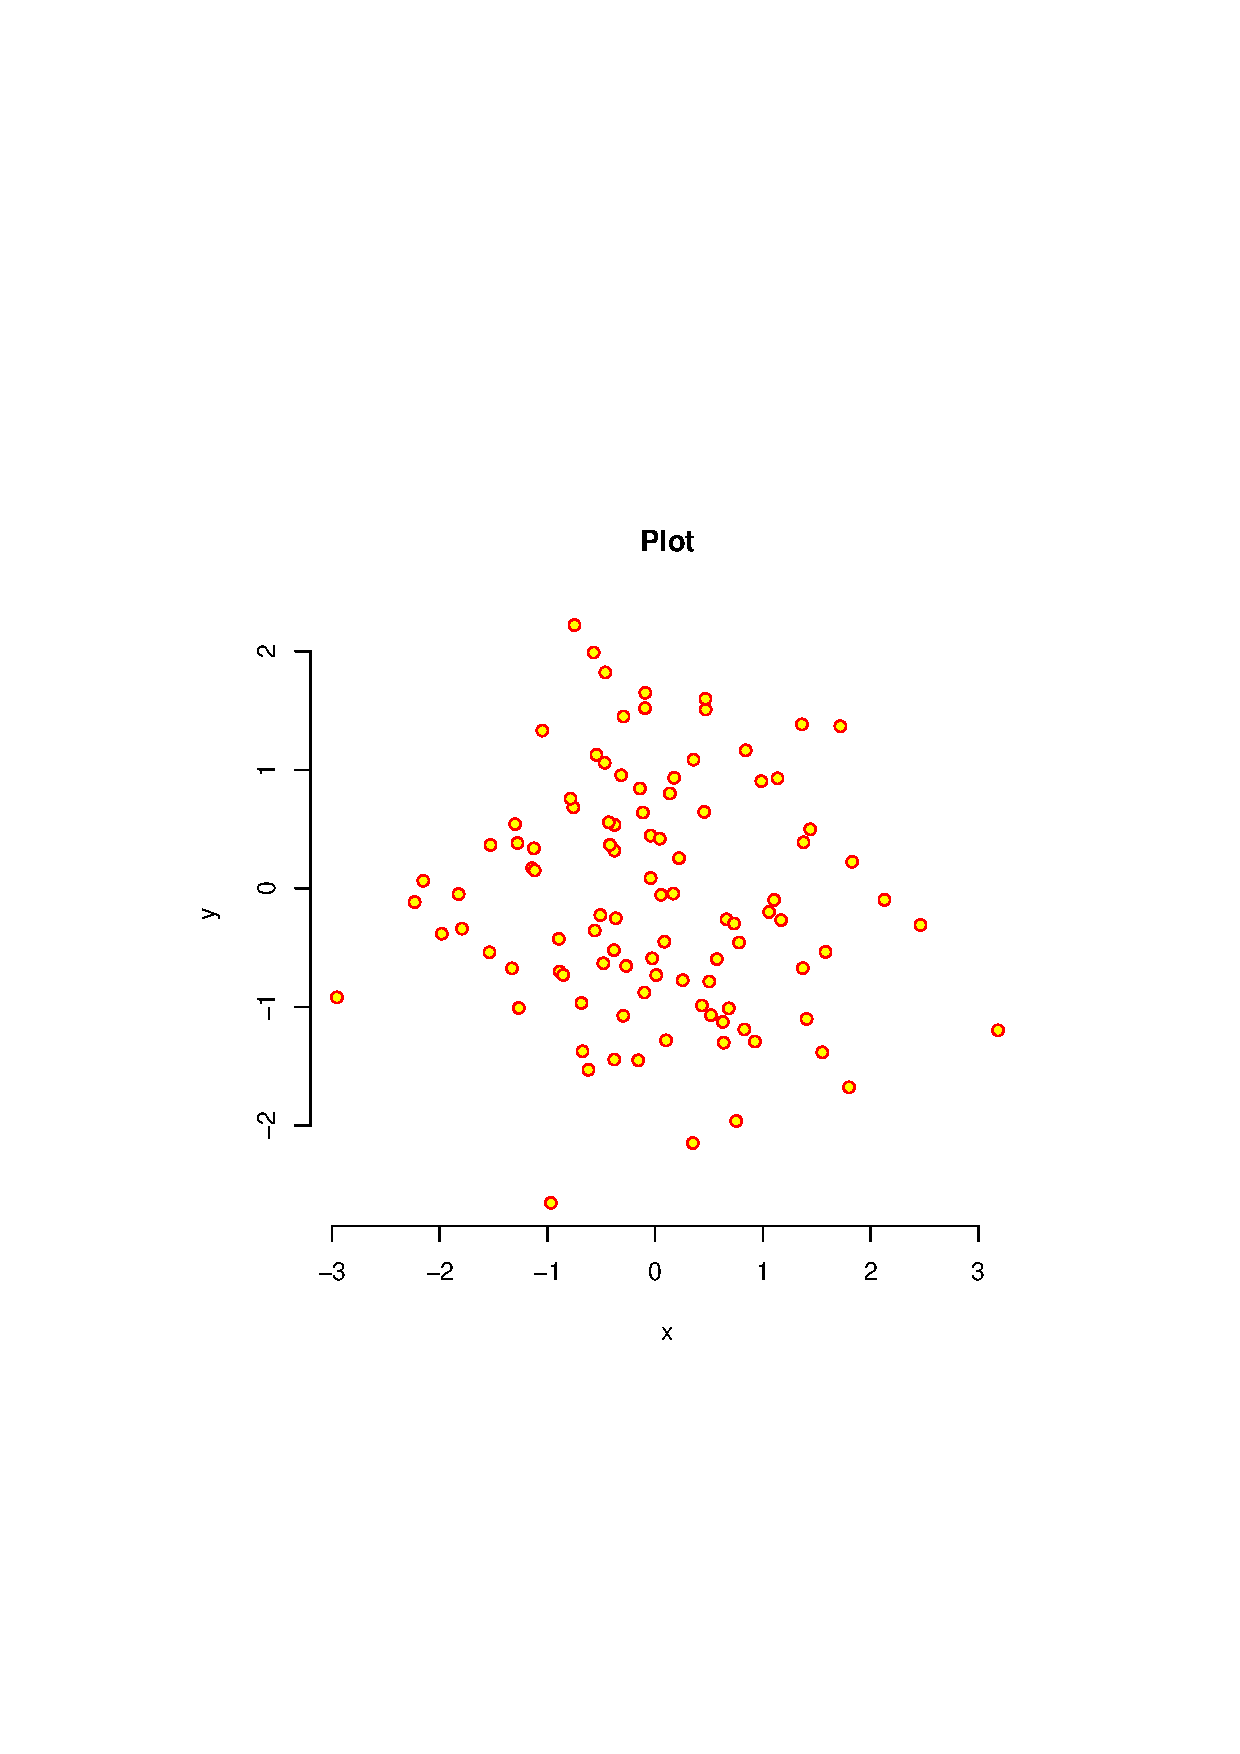
\includegraphics[width=6in, height=6in]{\FIGDIR/obr01}     
  %% příponu není potřeba explicitně uvádět, latex automaticky hledá
  %% ps/eps, pdflatex automaticky hledá pdf psfrag funguje pouze s
  %% ps/eps obrázky 
  
  \caption{Náhodný výběr z~rozdělení $\mathcal{N}_2(\boldsymbol{0},\,I)$.}
  \label{obr03:Nvyber}
  
  \end{figure}
  
  
  \begin{figure}[ht]\centering
  \label{obr03:Nhust}

  \psfrag{0.00}[c][c]{\textsf{0{,}00}}  
  \psfrag{0.02}[c][c]{\textsf{0{,}02}}  
  \psfrag{0.04}[c][c]{\textsf{0{,}04}}
  \psfrag{0.06}[c][c]{\textsf{0{,}06}}  
  \psfrag{0.08}[c][c]{\textsf{0{,}08}}
  \psfrag{m = 100, s = 15}[l][l]{\textsf{\large $\mu = 100,\; \sigma = 15$}}
  \psfrag{m = 110, s = 10}[l][l]{\textsf{\large $\mu = 110,\; \sigma = 10$}}
  \psfrag{m = 120, s = 5}[l][l]{\textsf{\large $\mu = 120,\; \sigma = 5$}}
  
  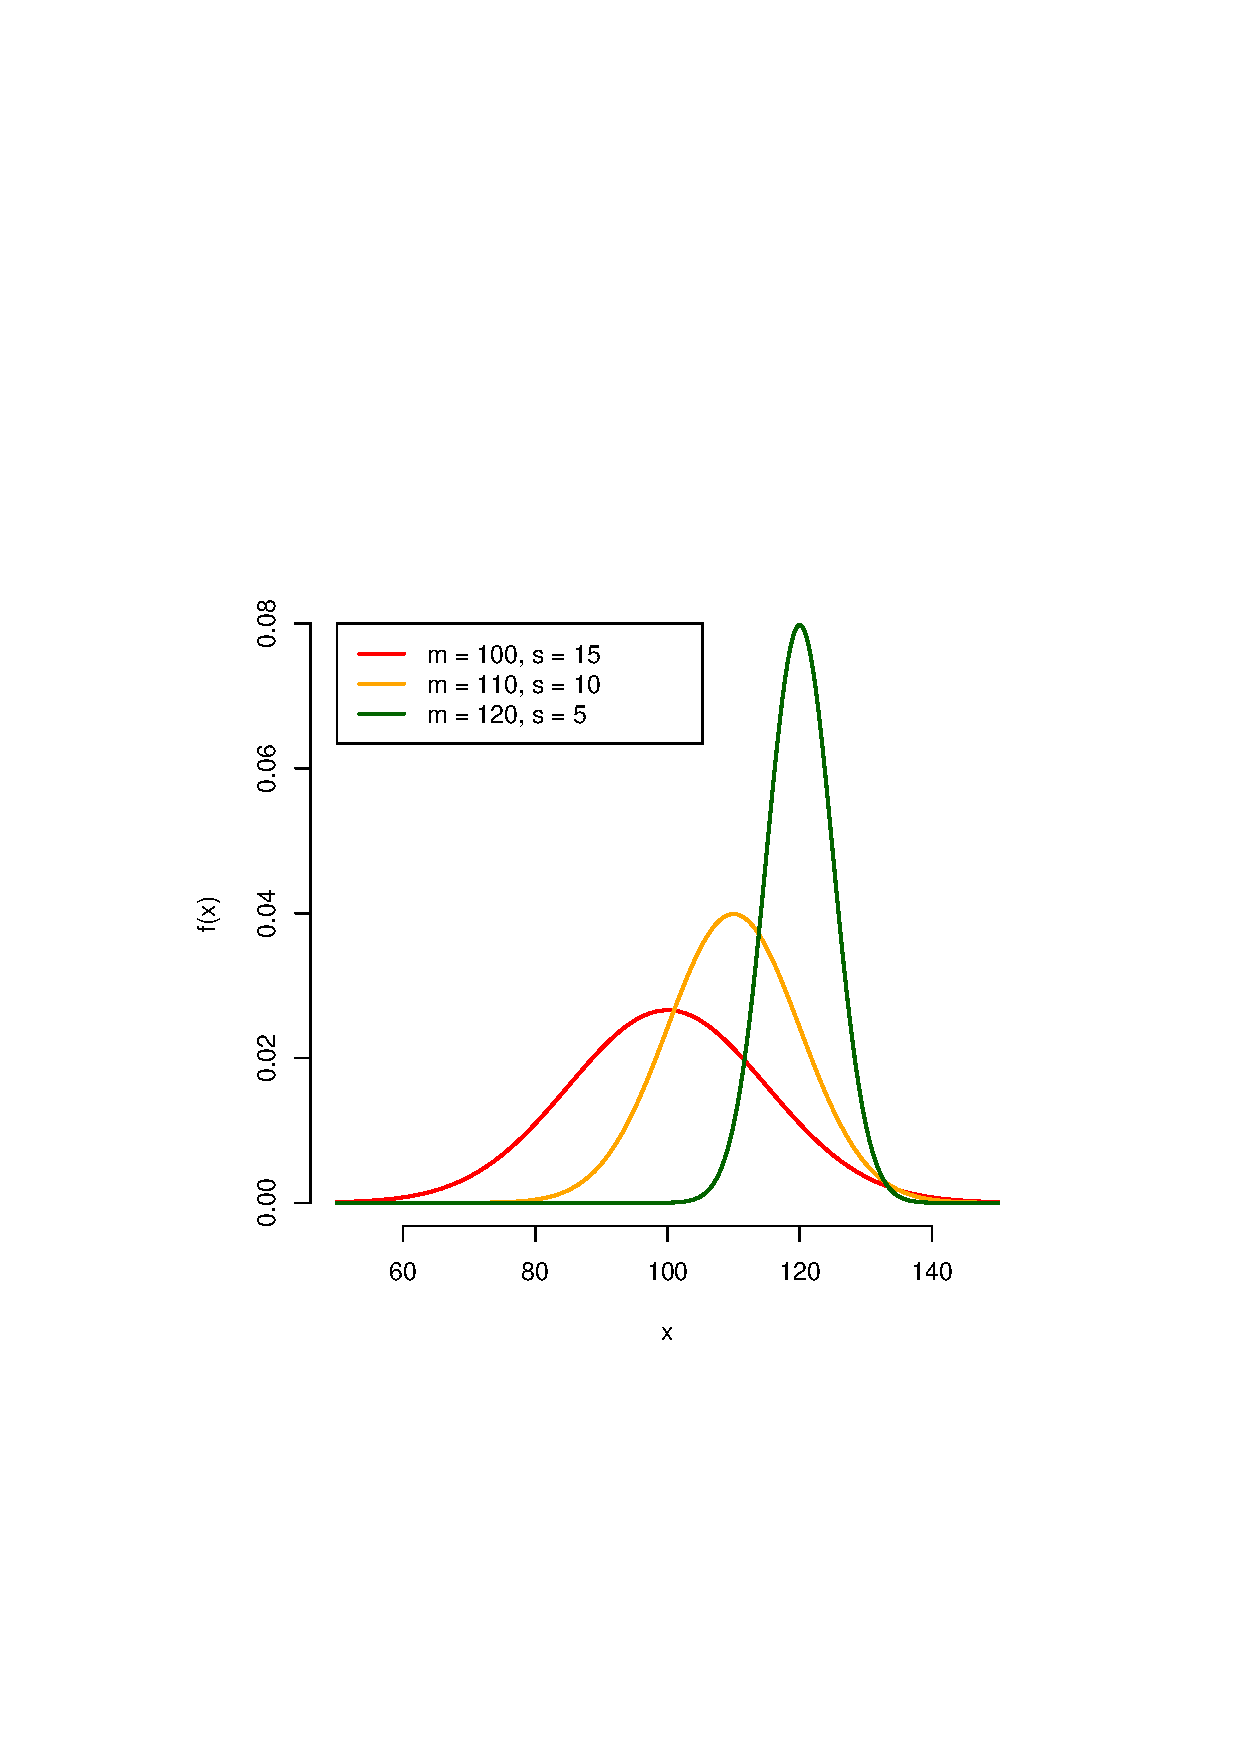
\includegraphics[width=6in, height=6in]{\FIGDIR/obr02}
  
  \caption{Hustoty několika normálních rozdělení.}
  
  \end{figure}
  
  
  % \begin{figure}[h]\centering
  % \psfrag{0.00}[c][c]{\textsf{\small 0{,}00}}  
  % \psfrag{0.02}[c][c]{\textsf{\small 0{,}02}}  
  % \psfrag{0.04}[c][c]{\textsf{\small 0{,}04}}
  % \psfrag{0.06}[c][c]{\textsf{\small 0{,}06}}  
  % \psfrag{0.08}[c][c]{\textsf{\small 0{,}08}}
  % \psfrag{60}[c][c]{\textsf{\small 60}}    
  % \psfrag{80}[c][c]{\textsf{\small 80}}  
  % \psfrag{100}[c][c]{\textsf{\small 100}}
  % \psfrag{120}[c][c]{\textsf{\small 120}}  
  % \psfrag{140}[c][c]{\textsf{\small 140}}
  % \psfrag{f\(x\)}[c][c]{\textsf{\small f(x)}}      
  % \psfrag{x}[c][c]{\textsf{\small x}}
  % \psfrag{m = 100, s = 15}[l][l]{\textsf{\large $\boldsymbol{\mu} \mathbf{\;= 100,}\; \boldsymbol{\sigma} \mathbf{\;= 15}$}}
  % \psfrag{m = 110, s = 10}[l][l]{\textsf{\large $\boldsymbol{\mu} \mathbf{\;= 110,}\; \boldsymbol{\sigma} \mathbf{\;= 10}$}}
  % \psfrag{m = 120, s = 5}[l][l]{\textsf{\large $\boldsymbol{\mu}  \mathbf{\;= 120,}\; \boldsymbol{\sigma} \mathbf{\;= 5}$}}
  
  % 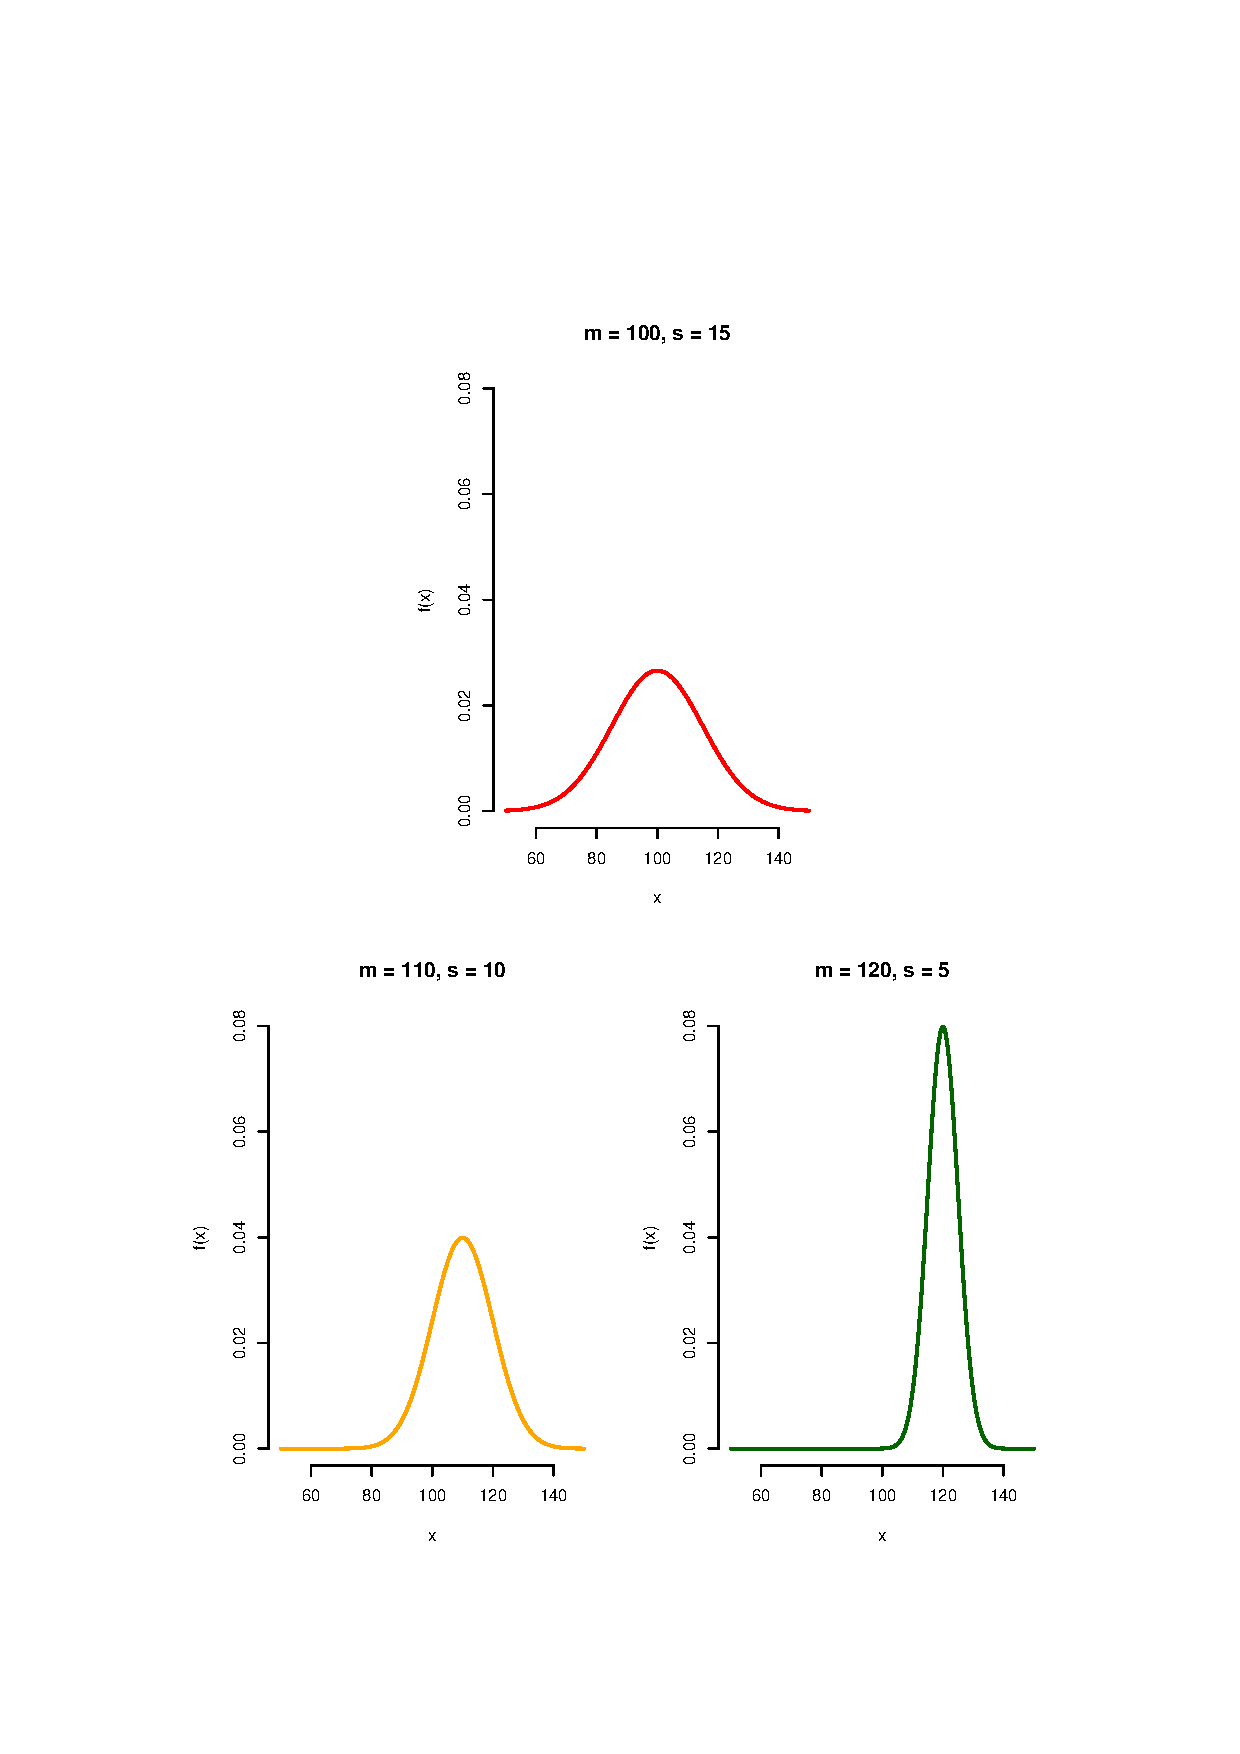
\includegraphics[width=6in, height=8.5in]{\FIGDIR/obr03}
  
  % \caption{Hustoty několika normálních rozdělení.}
  % \label{obr03:Nhust:podruhe}
  
  % \end{figure}




\section{Softwarový kód}

Softwarový kód, resp. výstupy z~počítačových programů (je-li potřeba
je v~práci uvádět) je vhodné odlišit od ostatního textu. Jednou
z~možností je použití {\LaTeX}o\-vé\-ho balíčku \texttt{fancyvrb}
(fancy verbatim), pomocí něhož je v~souboru \texttt{BcPrace.tex}
nadefinováno prostředí \texttt{PCinout}. Pomocí něho lze vytvořit
např. následující ukázky.
\begin{PCinout}
> mean(x)
[1] 158.90
> objekt\$prumer
[1] 158.90
\end{PCinout}
%$
Menší písmo:
\begin{PCinout}[fontsize=\footnotesize]
> mean(x)
[1] 158.90
> objekt\$prumer
[1] 158.90
\end{PCinout}
%$
Bez rámečku:
\begin{PCinout}[frame=none]
> mean(x)
[1] 158.90
> objekt\$prumer
[1] 158.90
\end{PCinout}
%$
Užší rámeček:
\begin{PCinout}[xrightmargin=20em]
> mean(x)
[1] 158.90
> objekt\$prumer
[1] 158.90
\end{PCinout}
%$



\newpage
\section{ukazka kodu}
\begin{lstlisting}
  class cell:
  ...
      def force_scalar(self, distance_between, direction, effect = True):
          epsilon = 0.0103
          sigma = 3.4
          return (48 * epsilon * np.power(sigma, 12) / np.power(distance_between, 13) - 24 * epsilon * np.power(sigma, 6) / np.power(distance_between, 7) * effect) * direction

      def energy_potential(self, distance_between, effect = True):
          epsilon = 0.0103
          sigma = 3.4
          return -4 * epsilon * np.power(sigma / distance_between, 6) * effect + 4 * epsilon * np.power(sigma / distance_between, 12)

      def find_centroid(self):
          # nalezeni teziste bunky, celkove hmotnosti a charakteru
          self.neutrals = 0
          self.particles_type = 0
          self.effect = 0
          self.N_particles = len(self.particles)
          if self.N_particles > 0:
              self.mass = 0
              self.centroid = np.array([0.0, 0.0, 0.0])
              for particle in self.particles:
                  self.centroid += particle.xyz*particle.mass
                  self.mass += particle.mass
                  self.particles_type += particle.particle_type
                  if particle.particle_type == 0:
                      self.neutrals += 1
              if self.particles_type != 0:
                  self.effect = self.particles_type / abs(self.particles_type)
              else:
                  self.effect = 0
              self.centroid = self.centroid/self.mass
          else:
              self.centroid = np.array([0.0, 0.0, 0.0])
              self.mass = 0
\end{lstlisting}


%%% Literatura 
%%% Reference se hledají v souboru priklady_literatury.bib. Aby se
%%% vytvořil seznam literatury, je třeba ocitovat alespoň jednu
%%% referenci, zkompilovat tento soubor latexem, pak bibtexem a znovu
%%% latexem. Tím se vytvoří seznam použitých referencí
%%% (BcPrace.bbl) a vloží se do práce na místě, kde se nachází příkaz
%%% \bibliography, tedy sem. 
%%% 
\bibliography{priklady_literatury}

%%% Obrázky v bakalářské práci, existují-li.
\listoffigures

%%% Tabulky v bakalářské práci, existují-li.
\listoftables

%%% Použité zkratky v bakalářské práci, existují-li, včetně jejich vysvětlení.
%\chapter*{Seznam použitých zkratek}
%\addcontentsline{toc}{chapter}{Seznam použitých zkratek}


%%% Přílohy k bakalářské práci, existují-li (různé dodatky jako výpisy programů,
%%% diagramy apod.). Každá příloha musí být alespoň jednou odkazována z vlastního
%%% textu práce. Přílohy se číslují.

%\chapter*{Přílohy}
%\addcontentsline{toc}{chapter}{Přílohy}



\end{document}

